\subsection{F.2.2 Calculate Train Position}\label{sss:calctrainpos}

\subsubsection{Short Description of Functionality}
The main purpose of the function is to calculate the locations of linked and unlinked balise groups (BGs) and the current train position while the train is running along the track. 

\begin{figure}[hbtp]
\centering
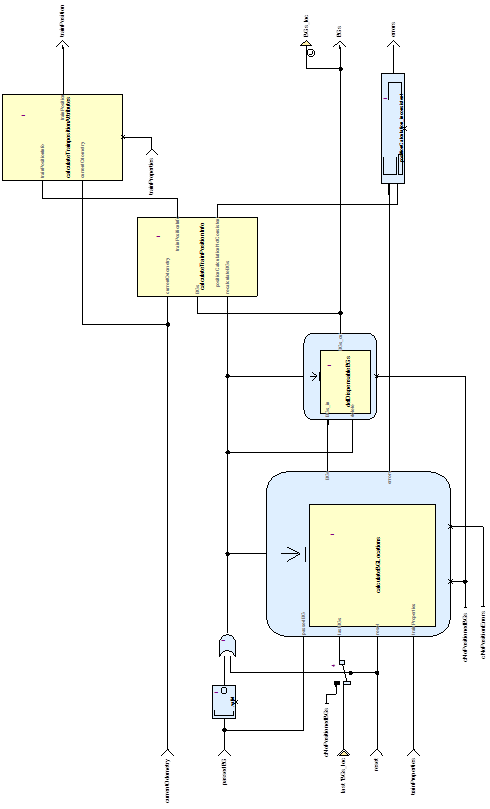
\includegraphics[scale=0.8]{../images/CalculateTrainPosition.png}
\caption{Structure of calculateTrainPosition}
\end{figure}


\paragraph{Functional Structure in Stages}
The function calculateTrainPosition is divided into the following four functions, which are being performed sequentially: 
\begin{enumerate}
\item \textbf{\textit{calculateBGLocations}}: Calculate the balise group locations\\
The first stage is triggered each time the train passes a balise group (input \textit{passedBG}). It takes the balise group header with the BG identification, the linking information (Subset 26, packet 5) and the current odometry values as inputs and calculates the location of the the passed balise group. If the passed BG has been announced via linking information previously, it takes into account the linking as well as the odometry information. If the passed BG does not meet the tolerance window announced by linking, an error flag is set. If the passed BG is an unlinked BG, its location is determined by odometry only, but related to the next previously passed linked BG, if there is one.\\
Then, if the passed BG is a linked BG comprising linking information for BGs ahead, the linking information is evaluated by creating the announced BGs and computing their locations from the linking distances.\\
The passed and the announced BGs are stored in a list \textit{BGs}, ordered by their nominal location on the track.\\
Afterwards the locations of all BGs are further improved by re-adjusting their locations with reference to the just passed BG. This optimizes the BG location inaccuries around the current train position (= location of the passed BG). 

\item \textbf{\textit{delDispensableBGs}}: Delete dispensable balise groups\\
The second stage removes balise groups supposed not to be needed any longer from the list of \textit{BGs}.\\
If the number of stored passed linked BGs exceeds the maximum number of eight as specified in \cite[Chapter~3.6.2.2.2 c]{subset-026}, all BGs astern are deleted.
If only (passed) unlinked BGs are in the list and exceed the number of \textit{cNoOfAtLeast\_x\_unlinkedBGs}, all passed BGs astern to those are removed from the list. 

\item \textbf{\textit{calculateTrainPositionInfo}}: Calculate train position information.\\
This stage take the list of stored BGs and the current odometry values as inputs and steadily provides the current train position. 

\item \textbf{\textit{calculateTrainpositionAttributes}}: Calculate train position attribute information.\\
This stage provides several additional position related attributes that might conveniently be used by subsequent consumers in the architecture.  
\end{enumerate}

\subsubsection{Reference to the SRS (or other requirements)}
The component calculateTrainPosition determines the location of linked and unlinked balise groups and the current train position during the train trip as specified mainly in \cite[Chapter~3.6]{subset-026}.

\subsubsection{Design Constraints and Choices}
The following constraints and prerequisites apply:
\begin{enumerate}
\item The input data received from the balises groups must have been checked and filtered for validity, consistency and the appropriate train orientation before delivering them to calculateTrainPosition. 
\item The storage capacity for balise groups is finite. calculateTrainPosition will raise an error flag when a balise group cannot be stored due to capacity limitations.
\item calculateTrainPosition will raise an error flag if a just passed balise group is not found where announced by linking information. It will not (yet) detect when an announced balise group is missing. 
\item calculateTrainPosition is not yet prepared for train movement direction changes. 
\item calculateTrainPosition does not yet consider repositioning information.
\end{enumerate}



\subsection{Provide Position Report}\label{sss:provposrep}

\begin{figure}[ht]
\centering
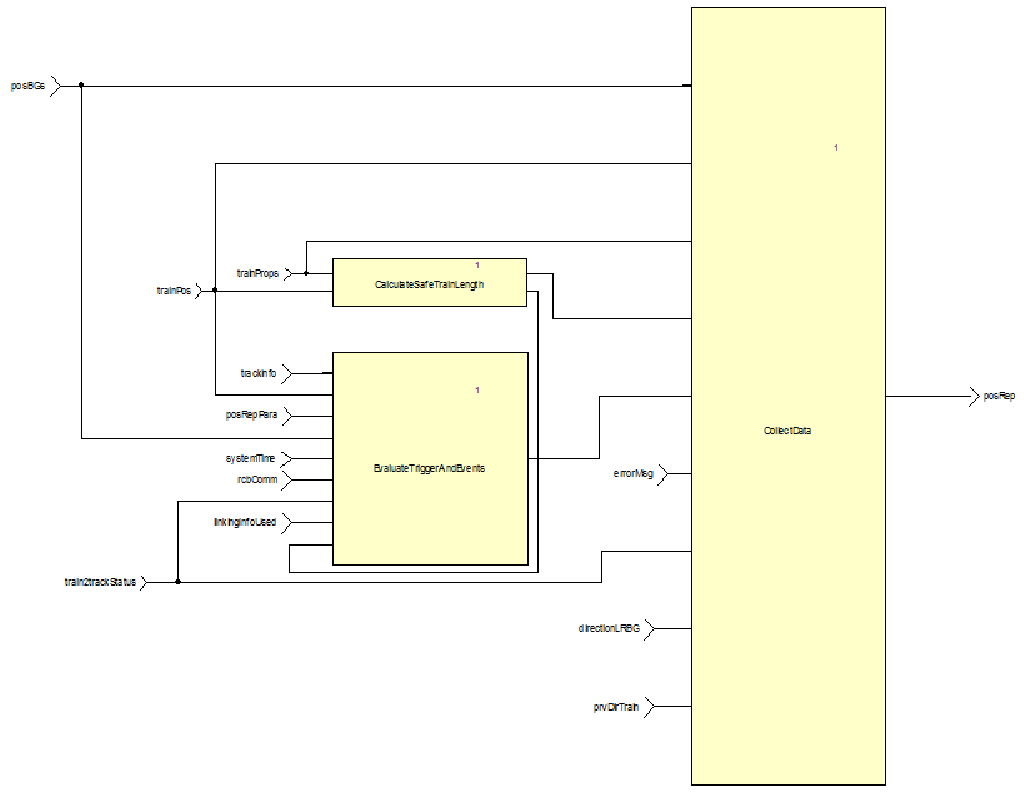
\includegraphics[width=\textwidth]{../images/ProvidePositionReport.pdf}
\caption{Structure of component ProvidePositionReport}\label{fig:provideposrep}
\end{figure}

\subsubsection{Short Description of Functionality}
This function takes the current train position and generates a position report which is sent to the RBC. The point in time when such a report is sent is determined by events, on the one hand, and position report parameters---which are basically triggers---provided by the RBC or a balise group passed, on the other hand. The functionality is modeled using three operations, as shown in Figure~\ref{fig:provideposrep}, which are explained below.
\begin{description}
	\item[CalculateSafeTrainLength] Calculates the the safeTrainLength and the MinSafeRearEnd according to \cite[Chapter~3.6.5.2.4/5]{subset-026}. \\
\verb+safeTrainLength =  absolute(EstimatedFrontEndPosition - MinSafeRearEnd)+, where
\verb+MinSafeRearEnd = minSafeFrontEndPosition - L_TRAIN+.
	\item[EvaluateTriggerAndEvents] Returns a Boolean modelling whether the sending of the next position report is triggered or not. This value is the conjunction of the evaluation of all triggers (PositionReportParameters, i.e., Packet 58) and events (see \cite[Chapter~3.6.5.1.4]{subset-026}).
	\item[CollectData] This operation aggregates data of Packet 0, \dots, Packet 5 and the header to a position report.
\end{description}

\subsubsection{Reference to the SRS (or other requirements}
Most of the functionality is described in \cite[Chapter~3.6.5]{subset-026}.

\subsubsection{Design Constraints and Choices}
\begin{enumerate}
	\item The message length (i.e., attribute \verb+L_MESSAGE+) is by default set to 0; the actual value will be set by the Bitwalker/API.
	\item The attribute \verb+Q_SCALE+ is assumed to be constant; that is, all operations using this attribute do not convert between different values of that attribute.
	\item \textit{PositionReportHeader}: The time stamp (i.e., attribute \verb+T_TRAIN+) is not set; this should be done once the message is being sent by the API.
	\item \textit{Packet 4}: When aggregating data for this packet, an error message might be overwritten by a succeeding error message. Because the specification allows only to sent one error in one position report, errors are not being stored in a queue, for instance.
	\item \textit{Packet 44}: This packet is currently not contained in a position report as it is not part of the kernel functions.
	\item The usage of attributes \verb+D_CYCLOC+ and \verb+T_CYCLOC+ as part of the triggers specified by the position report parameters (i.e., Packet 58 sent by the RBC) may lead to unexpected results if a big clock cycle together with small values for the attributes is used. The cause is that at every clock cycle the current model increments the reference value for the distance and time by at most \verb+D_CYCLOC+ and \verb+T_CYCLOC+, respectively and not a factor of it.
\end{enumerate}

\subsubsection{Open Issues}
\begin{enumerate}
	\item The specification requires to store the last eight balise groups for which a position report has been sent (see \cite[Chapter~3.6.2.2.2.c]{subset-026}).
	\item For all reports that contain Packet 1 (i.e., report based on two balise groups), the RBC sends a coordinate system. It is unclear where this has to be stored (i.e., somehow the balise groups have to be stored in a database which has then to be updated), see \cite[Chapter~3.4.2.3.3.6]{subset-026}. Moreover, such a coordination system can be invalid and then has to be rejected (see \cite[Chapter~3.4.2.3.3.7-8]{subset-026}). On a more abstract level, we need to think about the interface between the RBC and the OBU or a proper abstraction thereof.
\end{enumerate}
